\documentclass[11pt, a4paper]{article}
\usepackage[utf8]{inputenc}
\usepackage[T1]{fontenc}
\usepackage{amsfonts}
\usepackage{mathtools}
\usepackage{verbatim}
\usepackage{float}
\usepackage{graphicx}
\usepackage{times}  
\usepackage{tocbibind}
\usepackage[lined, boxed, linesnumbered]{algorithm2e}
\usepackage{array}
\usepackage{makecell}
\usepackage{tikz}
\usepackage{amsthm}
\usepackage{lscape}
\usepackage{caption}
\usepackage{subcaption}
\usepackage{subfig}

\title{CMP155 - An\'{a}lise e Desenvolvimento de Algoritmos}
\author{Leonardo Fernando dos Santos Moura}

\begin{document}

\maketitle

\section{Introduction} 
%motivation for the choice of this particular article
To this assignment I chose the article VNE-AC: Virtual Network Embedding Algorithm Based on Ant Colony Metaheuristic \cite{fajjari2011}. It is one of the few implementations of metaheuristics to this class of problems.

This article was published on the 2011 IEEE International Conference on Communications (ICC). That conference has a Qualis rating of A2. According to Google it was cited 23 times, and 5, according to IEEEXPLORE.
%the authors
Its authors work mainly on the areas of high-speed and wireless networks, cloud computing and network virtualization. Ilhen Fajjari and Guy Pujolle are involved in the startup VirtuOR, based on France, that provides network virtualization solutions.

% TODO: motivation for virtual networks
Network virtualization consists in running multiple virtual networks on a physical substrate infrastructure. It has been recognized as a way of overcoming the resistance to change offered by the protocols of the Internet \cite{lu}. Virtual networks are also used to test new protocols.

\section{Problem Definition}
The problem of virtual network embedding consists in mapping virtual networks on a physical substrate, optimizing the allocation of resources and the number of virtual network requests along a defined time scale. A virtual vertex has to be mapped to a substrate vertex that has enough resources. A virtual link has to be mapped to a path in the substrate infrastructure. This path has to be valid, have enough resources and join the two virtual vertices of the link.

Each virtual node must be mapped to a single substrate vertex, and each substrate vertex can have only one virtual vertex of the same virtual network request mapped to it.

The vertices are classified as ``access'' or ``core''. Access nodes are those at which traffic enters or exits the network. A virtual access vertex has to be mapped to a substrate access vertex. 

A substrate network is modelled as an undirected graph $SN = G^{S}(N^{S}, E^{S})$. The set of vertices in the substrate network are represented by $N^{S}$ and the set of links between those vertices are represented by $E^{S}$. Each vertex $i$ has a residual processing power $C_{n^{S}_{i}}$, residual memory $M_{n^{S}_{i}}$, a geographic location $L_{n^{S}_{i}}$ and a type, that can be either ``access'' or ``core''. Each link has a residual bandwidth capacity $B_{e^{S}_{i}}$. Similarly the virtual network is defined as an undirected graph with requirements of processing power and memory, and of bandwidth for its links. Also, in the virtual network, the vertices have a location and they must be mapped within a radius $D$ of that location.

In Figure~\ref{example}, an example of an instance is shown. On the left there is the substrate graph with its access and core nodes. On the right there is on virtual network composed of four nodes.

\begin{figure}[h]
  \centering
  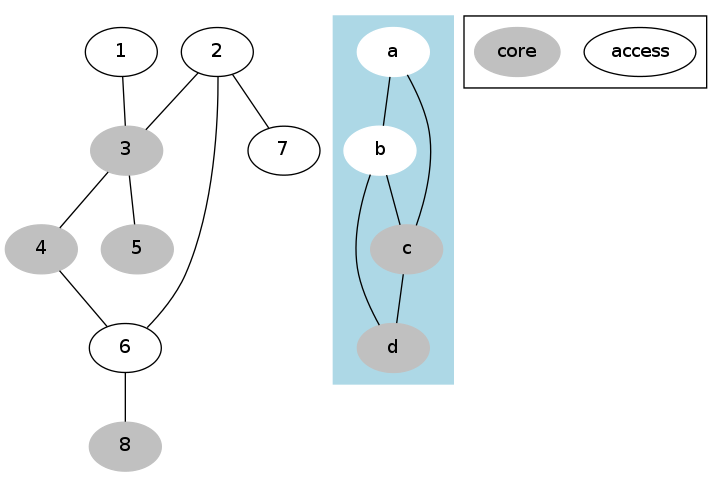
\includegraphics[scale=0.35]{g1.png}
  \caption{Virtual Network Embedding Instance Example }\label{example}
\end{figure}

Since the processing power and memory are fixed and cannot be reduced with a better mapping, the main objective of a specific mapping of a virtual network is to minimize the sum of the bandwidth used by this network.

\section{Algorithm}
The article proposes a Max Min Ant Colony System to solve the given problem. This type of metaheuristic is based on nature: a set of independent ants construct randomly a solution, the best one reinforces a pheromone trail, which other ants might follow.

The process is summarized in Algorithm~\ref{algo}. First the access nodes are mapped greedily: the virtual access vertices are mapped to the substrate vertices that have the most residual resources. The links between access vertices are mapped using the process described in Section~\ref{path}. Then the problem of mapping the virtual core nodes is divided into subproblems called components. Each component correspond to a virtual core node and its ``hanging links''. A hanging link is a virtual link that has one of its adjacent vertices already mapped. The components are sorted according to number of hanging links. After all components are constructed the heuristic search begins. Each independent ant maps the vertices corresponding to the components randomly using the probabilities defined by its pheromone trail. At the end of each iteration the pheromone trail is evaporated and the decisions corresponding to the best solution are reinforced. So at the end, the decisions that led to better solutions will have an increasingly bigger probability of being selected.

\begin{algorithm}
  \ForEach{Access node $v$ in the virtual network $VN$}
  {map $v$ to the substrate access vertex with most resources\;
   map all virtual links between access vertices\;
   remove $v$ and its mapped links from $VN$}
  \While{$VN$ is not empty} 
  {get the vertex $u$ with most hanging links\;
   remove $u$ and all its hanging links from $VN$ and create a component;
  }
  \For{$i := 1$ to $N_{iter}$}
  {\For{$ant := 1$ to $A_{ants}$}
    {map components\;}
    update pheromone trail\;
  }
\caption{ACO for the network embedding problem}
\label{algo}
\end{algorithm}

Each component has a set of candidate $PNa$ substrate vertices that it can be mapped to. The candidates are those vertices with enough resources that are located within $H$ hops of the barycenter of the vertices at the end of the hanging links. The probability of a given vertex $a$ being mapped into $b$ is given by the following equation:
\begin{equation}
  p_{ab} = \frac{\tau^{\alpha}_{ab} \eta^{\beta}_{ab}}
  {\sum_{b \in PN_{a}} \tau^{\alpha}_{ab} \eta^{\beta}_{ab}}
\end{equation}

Where $\tau$ is the pheromone trail, and $\eta$ is the heuristic information. The parameters $\alpha$ and $\beta$ dictate the weight given to the pheromone and heuristic information, respectively. 

The heuristic information is calculated at the beginning of the algorithm and is defined as:
\begin{equation}
  \eta_{ab} = C_{n^{S}_{b}} + M_{n^{S}_{b}} + \sum_{k \in N_{a}} B_{P_{bk}}
\end{equation}

The heuristic information is the sum of the residual processing power and memory of $b$ and the sum of the costs of the best paths (according the metric defined in~\ref{metric}) between $b$ and all the substrate vertices in which the hanging links of $a$ were mapped. 

The pheromone trail is updated at the end of each iteration. All the values of $\tau$ are reduced by multiplying them by the parameter $\rho \in (0,1)$. If the component $a$ was mapped into substrate vertex $b$ in the best solution, $\tau_{ab}$ is reinforced so that the probability of it being selected again increases. The exact update function is defined below:

\begin{equation}
  \tau_{ab}(t+1) = \left\{  
  \begin{array}{l l}
    \rho \tau_{ab}(t) + \frac{\phi}{best solution cost} & \text{if $a$ was mapped to $b$ in the}\\
                                                        & \text{best solution of iteration $t$} \\
    \rho \tau_{ab}(t) & \text{otherwise}
  \end{array}\right .
\end{equation}

If all values of pheromone are large, the search will be fairly random. Otherwise if the values are small, the search will be greedy. To balance those values, the pheromone trail values are locked between the interval $[\tau_{min},\tau_{max}]$. Every $\tau_{ab}$ is initially set to $\tau_{max}$ to start the algorithm with a random search, obtaining a better pheromone information.

\subsection{Mapping Virtual Links} \label{path}
The best path between two substrate nodes is the one that spend less bandwidth of the network. In the article the author suggests the following metric:

\begin{equation}
  d(P) = \frac{lenght(P)}{\min_{e^{S}_{x}\in P}B_{e^{S}_{x}}}\label{metric}
\end{equation}

To find the best path using this metric I used Dijkstra shortest path algorithm using a priority queue, that has a time complexity of $O(|E| log |V|)$.

\subsection{Validation}
Since the instances are generated randomly and there are no known implementation of this particular problem, I developed my own procedures to validate the final solution. The validation procedure checks if every virtual node was mapped to a different substrate node with enough resources, if all the virtual links were mapped to a valid path on the substrate graph. Also  it is checked whether the cpu, memory and bandwidth resources where in fact used after an virtual network allocation and freed after the requests finishes.

\section{Results}
\subsection{Instances Generation}
Instances were generated using the \texttt{GT-ITM} tool. The graphs were generated using the Waxman model \cite{waxman88}. Two vertices $u, v$ in a graph are linked with probability $P(u,v)$ defined in Equation~\ref{waxman}, where $L$ is the maximum distance between any two nodes. The bigger the $\alpha$, more edges the graph will have. An increasing in $\beta$ will increase the number of long edges.

\begin{equation}
  P(u,v) = \alpha e^{-rand(0,L)/(\beta L)} \label{waxman}
\end{equation}

Both the substrate and the virtual networks were generated using $\alpha = 0.5$ and $\beta = 0.2$. The substrate graph has 100 vertices, with 20\% of those being access vertices. The virtual graphs sizes are distributed uniformly in the interval $[2,10]$, with 50\% of them being access vertices. The substrate resources (processing power, memory and edge bandwidth) are distributed uniformly in the interval $[50,100]$, whereas the required resources on the virtual networks are distributed in the interval $[10,20]$.

The way of distributing the access and core nodes was not specified in the article so the vertices were set randomly to access with probability $0.2$, for the substrate graph, and $0.5$, for the virtual network graphs.

In the simulation, the arrival of new requests is modelled as a Poisson process with a rate $\lambda$ of 4 requests per 100 time units and with requests having a lifetime modeled as an exponential distribution with mean $\mu$ of 1000 time units. The simulation is run over 2000 requests.

\subsection{ACO parameters}
The number of ants was set to 10 and the number of iterations was set to 20. The hop-range $H$ was set to 3. The importance of the heuristic and pheromone trail, $\alpha$ and $\beta$, was set to 1 and 2 respectively. Since the value of $\tau_{max}$ and $\tau_{min}$ was not specified in the paper I used the values 130 and 1, respectively. The radius $D$ also was not specified, so it was set to infinity.

As for the parameter $\phi$, it was not clear what is its role in the search. A large value would overestimate the value of the choices of mappings in one given iteration. So I chose to set is as $1$.

\subsection{Results}
I unfortunately could not reproduce the results shown in the article. All requests that are rejected are so due to the exhaustion of the substrate access nodes. Doing a back of the envelope calculation one can reach to the conclusion that the substrate graph will have on average a total of 1500 units of processing power and memory, and after a thousand time units, the network requests will require 1800 units. Since there are also the problem of fragmentation (some substrate vertices will have less processing power than any requested one). We can estimate that at least 20\% percent of the requests will be rejected using the parameters I used, whereas in the article the authors achieve around 4.5\%.

Figure~\ref{cpu} shows the minimum amount of cpu in access vertices necessary to accept every request in one run of the simulation in function of the time. The red line crossing the graph is the amount of cpu in the substrate graph used in this simulation. As it can be seen, the amount of cpu surpasses the line, so it is impossible to accept every request.

\begin{figure}[h]
  \centering
  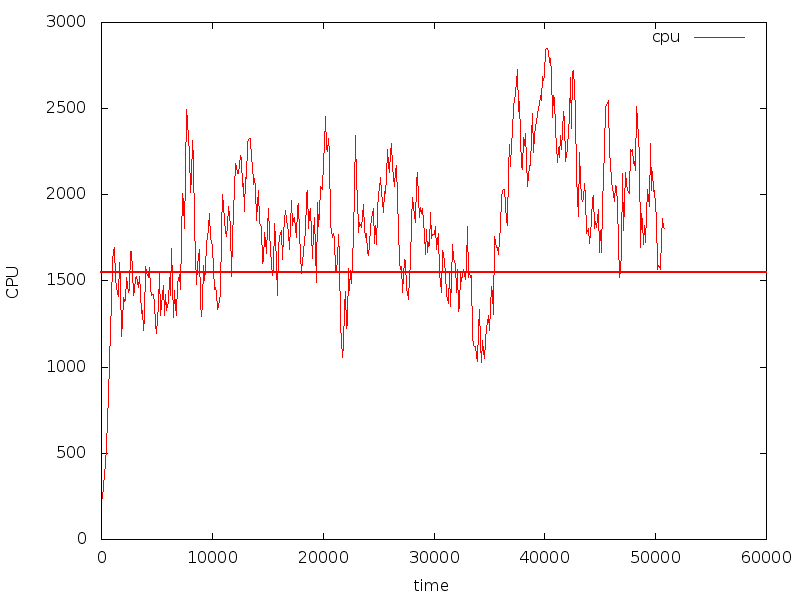
\includegraphics[scale=0.35]{cpu.png}
  \caption{Lower Bound on the Processing Power needed in order to accept all requests}\label{cpu}
\end{figure}

Figure~\ref{reject} shows the reject rate of single run of the simulation, the final reject rate obtained was around 25\%. I ran it a few times with randomly generated graphs and the reject rate did not differ much from this rate.

\begin{figure}[h]
  \centering
  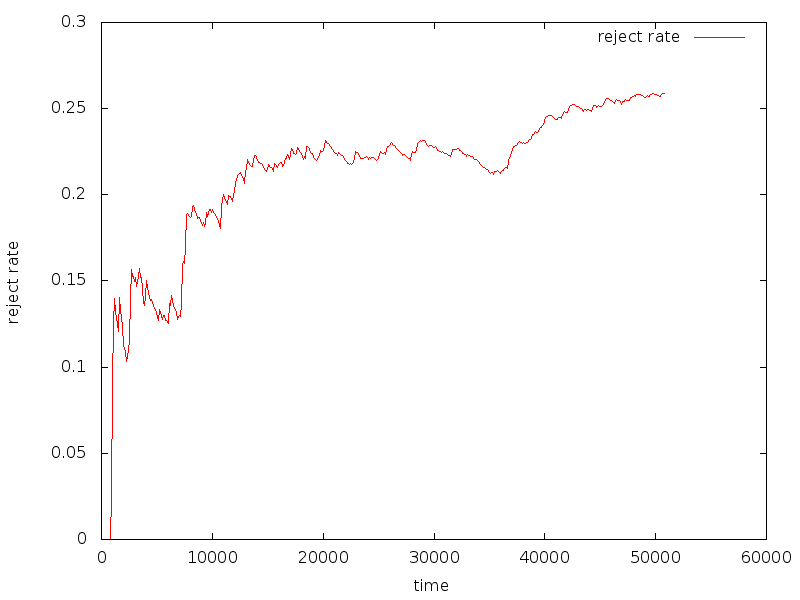
\includegraphics[scale=0.35]{rejectrate.png}
  \caption{Reject Rate}\label{reject}
\end{figure}

\section{Conclusion}
Although the results obtained were not the same as the ones obtained in the article, it was interesting to implement this fairly complex algorithm. Some parameters used and the exact methods by which the graphs were generated were missing. Also the details of the requirements of the simulation (the relation between different virtual networks mapped on the same substrate) were implicit, making the procedure harder to reproduce. The choice of parameters could also be explored a little more, the authors just state that they were obtained ``based on extensive simulations''.

I learned, as I think it was this assignment goal, that the problem has to be formally explained and that all parameters have to be clearly specified.

As a suggestion for improvement of the method employed in the article, the heuristic search could be expanded to the choice of mapping the access vertices instead of mapping them greedily. Randomization could also be used, a multi start algorithm would be easy to implement.

\bibliography{design}
%\bibliographystyle{abnt}
\bibliographystyle{plain}

\end{document}
